\subsection*{Aufgabe 3}

Die beiden Funktionen in Abbildung \ref{fig:f} sollen integriert werden. Dafür werden Integrationsroutinen für die Mittelpunkts-, Trapez- und Simpsonregel implementiert.
\begin{figure}[H]
    \centering
    \begin{subfigure}[b]{0.45\textwidth}
        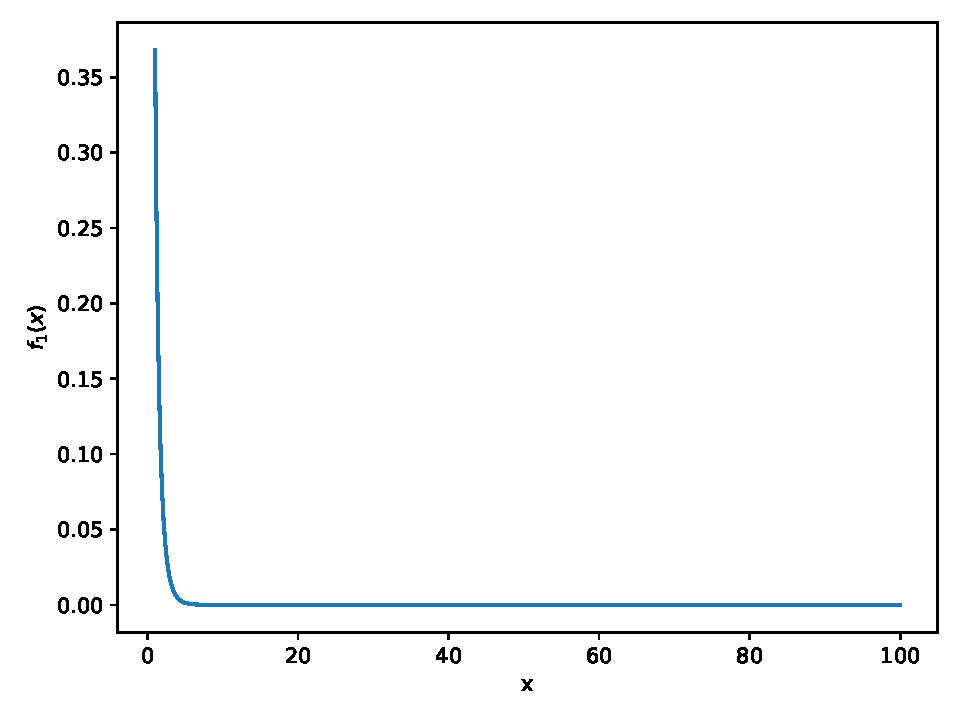
\includegraphics[width=\textwidth]{A3/build/f1.pdf}
        \caption{Funktion \(f_1(x) =  \frac{e^x}{x}\).}
        \label{fig:f1}
    \end{subfigure}
    ~ %add desired spacing between images, e. g. ~, \quad, \qquad, \hfill etc.
    %(or a blank line to force the subfigure onto a new line)
    \begin{subfigure}[b]{0.45\textwidth}
        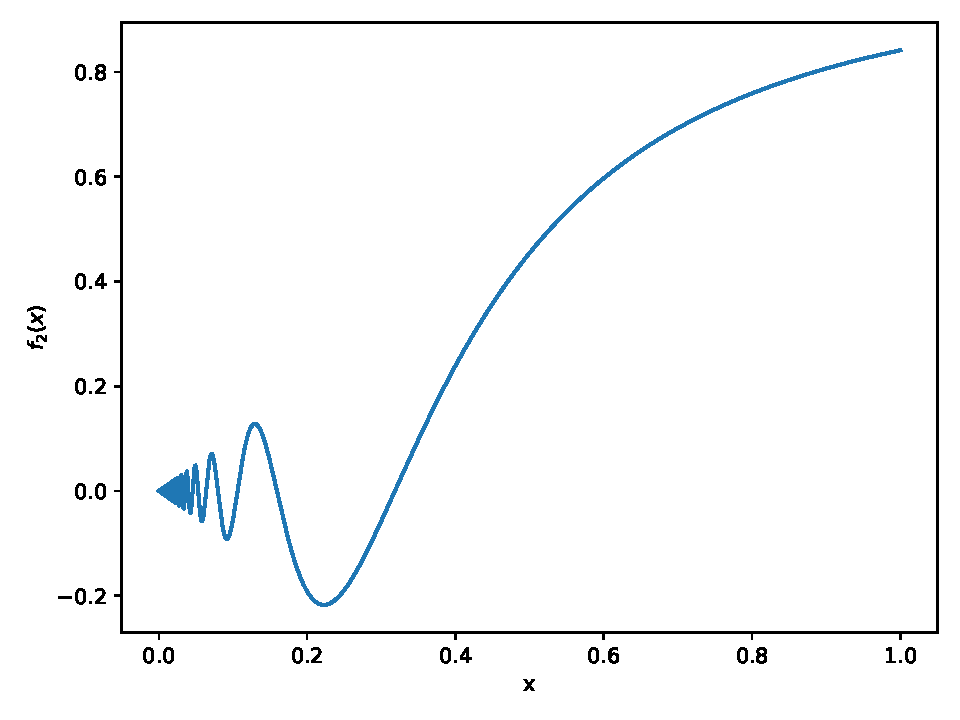
\includegraphics[width=\textwidth]{A3/build/f2.pdf}
        \caption{Funktion \(f_2(x) = x \sin{\left(\frac{1}{x}\right)}\).}
        \label{fig:f2}
    \end{subfigure}
    \caption{Zu integrierende Funktionen.}\label{fig:f}
\end{figure}

Die Integrationsroutinen sollen nun getestet werden, indem die Intervallbreite \(h\) halbiert wird bis die relative Änderung der Ergebnisse kleiner als \(\num{1e-4}\) ist.
Wie in den Abbildungen \ref{fig:I1} und \ref{fig:I2} zu sehen ist, werden dafür die relative Änderung \(\varepsilon_\text{rel.}\) gegen die Intervallzahl \(n\) aufgetragen.
Mit \(n\) ergibt sich die Intervallbreite zu
\begin{equation*}
  h = \frac{b-a}{n}
\end{equation*}
\begin{center}
  \tiny{\(a \: \hat{=}\) untere Integralgrenze, \(b \: \hat{=}\) obere Integralgrenze}
\end{center}
die Verdopplung der Intervallzahl bewirkt also eine Halbierung der Intervallbreite.
Die relative Änderung des Ergebnisses ergibt sich aus
\begin{equation*}
  \varepsilon_\text{rel.} = \frac{\left|y_\text{alt} - y_\text{neu} \right|}{y_\text{alt}}.
\end{equation*}

In Abbildung \ref{fig:I1} sind die relativen Änderungen für das Integral \(I_1\) dargestellt
\begin{equation*}
  I_1 = \int_1^{100} \frac{e^{-x}}{x} \mathrm{d}x.
\end{equation*}
Der Verlauf ist bei der Trapez- und Mittelpunktsregel sehr ähnlich. Zu Beginn sind die relativen Abweichungen sehr groß und ändern sich stark. Zu hohen \(n\) ändern sich die Abweichungen nur noch leicht.
Bei der Simpsonregel ist die relative Abweichung zu Beginn ziemlich konstant bei ungefähr \(1\) und fängt erst bei \(2^7\) Teilintervallen an kleiner zu werden.
Damit die relative Änderung bei der Trapezregel auf unter \(\num{1e-4}\) fällt muss das Intervall \([1,100]\) in \(2^{20}\) Teilintervalle aufgeteilt werden, dies entspricht einer Intervallbreite von \(h=\num{9,44e-5}\).
Bei der Mittelpunktsregel ist dies bei \(2^{13}\) Teilintervallen, also \(h=\num{0,01}\), der Fall.
Am schnellsten wird der Wert allerdings von der Simpsonregel bei nur \(2^{11}\) Teilintervallen bzw. \(h=\num{0,05}\) erreicht.

\begin{figure}
  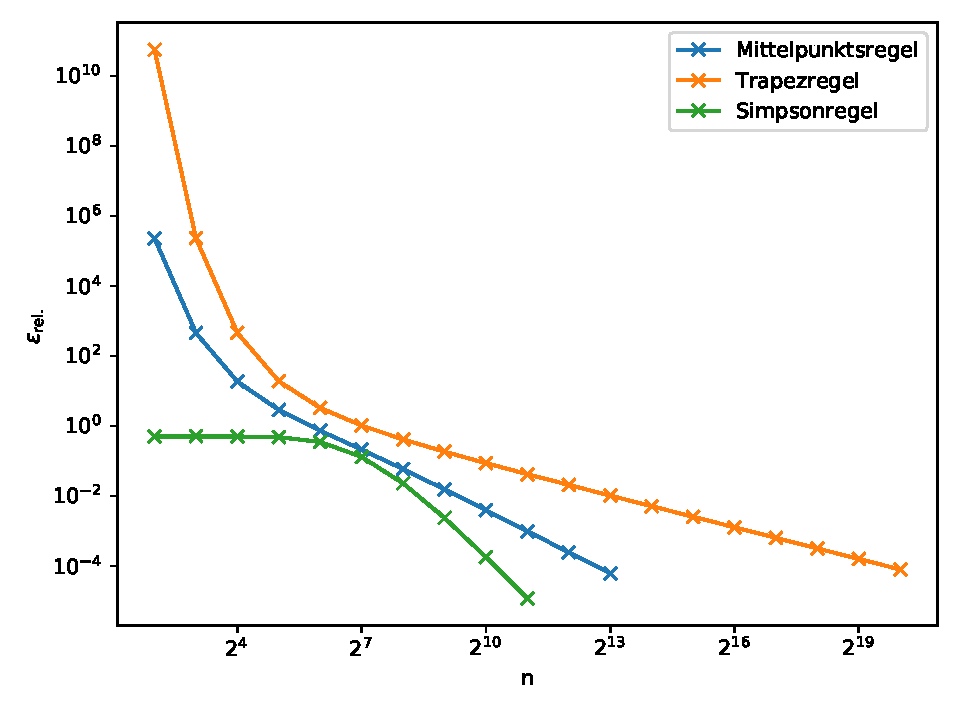
\includegraphics[width=0.8\textwidth]{A3/build/I1.pdf}
  \caption{Vergleich der relativen Änderungen für Integral \(I_1\).}
  \label{fig:I1}
\end{figure}

In Abbildung \ref{fig:I2} sind die relativen Änderungen für das Integral \(I_2\) dargestellt
\begin{equation*}
  I_2 = \int_0^1 x \sin{\left(\frac{1}{x} \right)} \mathrm{d}x.
\end{equation*}
Was direkt auffällt ist, dass die relativen Abweichungen insgesamt viel kleiner sind. Dies liegt an dem kleineren Intervall und der damit automatisch kleineren Intervallbreite.
Auch hier sind die relativen Abweichungen bei der Trapezregel am höchsten und es werden die meisten Teilintervalle \(2^{14}\) (\(h=\num{6,10e-5}\)) benötigt, um unter die Vorgabe von \(\num{1e-4}\) zu kommen.
Außerdem ist auffällig, dass die relative Abweichung bei der Mittelpunktsregel zwar auf einem deutlich geringerem Niveau beginnt aber zunächst ansteigt bevor sie bei \(2^5\) Teilintervallen (\(h=\num{0,03}\)) zu sinken beginnt.
Dadurch ist die benötigte Anzahl an Teilintervallen bei Mittelpunkts- und Simpsonregel gleich groß bei \(2^8\) (\(h=\num{3,9e-3}\)).
Allerdings ist bei der Simpsonregel die relative Abweichung nach erreichen des Grenzwertes kleiner, weshalb auch bei \(I_2\) die Simpsonregel vorzuziehen ist.

\begin{figure}
  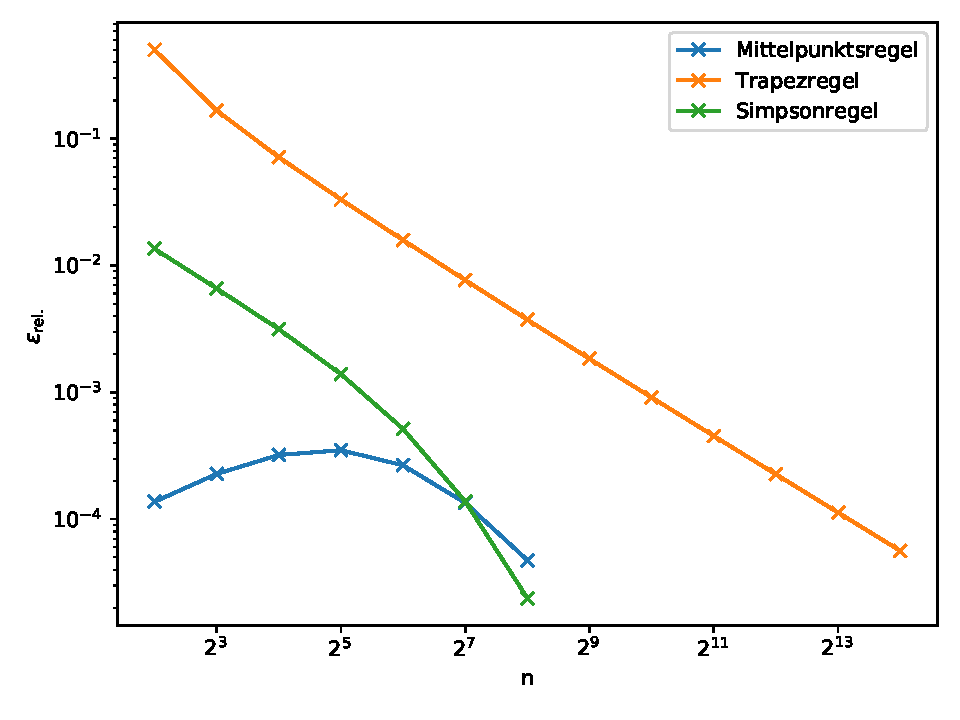
\includegraphics[width=0.8\textwidth]{A3/build/I2.pdf}
  \caption{Vergleich der relativen Änderungen für Integral \(I_2\).}
  \label{fig:I2}
\end{figure}

\FloatBarrier
